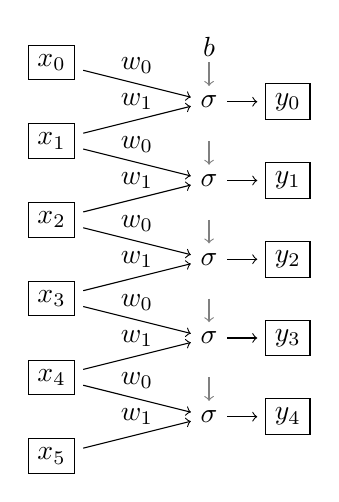
\begin{tikzpicture}[main/.style = {draw, outer sep=3pt}] 
    \node[main] (x0) at (0, 0)  {$x_0$}; 
    \node[main] (x1) at (0, -1) {$x_1$};
    \node[main] (x2) at (0, -2) {$x_2$}; 
    \node[main] (x3) at (0, -3) {$x_3$};
    \node[main] (x4) at (0, -4) {$x_4$}; 
    \node[main] (x5) at (0, -5) {$x_5$};

    \node (y0) at (2, -0.5) {$\sigma$};
    \node (y1) at (2, -1.5) {$\sigma$};
    \node (y2) at (2, -2.5) {$\sigma$};
    \node (y3) at (2, -3.5) {$\sigma$};
    \node (y4) at (2, -4.5) {$\sigma$};

    \node[main] (yy0) at (3, -0.5) {$y_0$};
    \node[main] (yy1) at (3, -1.5) {$y_1$};
    \node[main] (yy2) at (3, -2.5) {$y_2$};
    \node[main] (yy3) at (3, -3.5) {$y_3$};
    \node[main] (yy4) at (3, -4.5) {$y_4$};

    \draw [->] (x0) -> node[above, align=center] {$w_0$} (y0);
    \draw [->] (x1) -> node[above, align=center] {$w_1$} (y0);
    \draw [->, gray] (y0) + (0,0.5) -> node[above=3pt, align=center, black] {$b$} (y0);
    \draw [->] (y0) -> (yy0);

    \draw [->] (x1) -> node[above, align=center] {$w_0$} (y1);
    \draw [->] (x2) -> node[above, align=center] {$w_1$} (y1);
    \draw [->, gray] (y1) + (0,0.5) -> node[above=1pt, align=center] {} (y1);
    \draw [->] (y1) -> (yy1);


    \draw [->] (x2) -> node[above, align=center] {$w_0$} (y2);
    \draw [->] (x3) -> node[above, align=center] {$w_1$} (y2);
    \draw [->, gray] (y2) + (0,0.5) -> node[above=1pt, align=center] {} (y2);
    \draw [->] (y2) -> (yy2);


    \draw [->] (x3) -> node[above, align=center] {$w_0$} (y3);
    \draw [->] (x4) -> node[above, align=center] {$w_1$} (y3);
    \draw [->, gray] (y3) + (0,0.5) -> node[above=1pt, align=center] {} (y3);
    \draw [->] (y3) -> (yy3);


    \draw [->] (x4) -> node[above, align=center] {$w_0$} (y4);
    \draw [->] (x5) -> node[above, align=center] {$w_1$} (y4);
    \draw [->, gray] (y4) + (0,0.5) -> node[above=1pt, align=center] {} (y4);
    \draw [->] (y4) -> (yy4);

\end{tikzpicture} 
